\section{Scene Construction}
\label{chapter:design:scenegraph}

	Scene graphs are opaque in all of the reference engines, requiring the designer of a scene to use these constructs explicitly when constructing a scene. Panda3d declares that a \classname{Model} is merely a special \classname{SceneNode} that can handle rotating, movement and scaling, while Ogre3d considers \classname{Model}s to be \classname{Object}s and moves them outside the scene graph hierarchy. OpenSceneGraph takes an even stricter approach and defines that such operations can only be performed on nodes dedicated to these tasks.

	Creating a port of the scene depicted in Figure \ref{fig:ExampleSceneGraph} in Ogre3d could look as follows:

	\begin{code}[2]
		// create scene nodes
		tableRootNode = roomNode->createChildSceneNode("TableRootNode")
		tableNode = tableRootNode->createChildSceneNode("TableNode")
		cutleryNode = tableNode->createChildSceneNode("CutleryNode")
		forkNode = cutleryNode->createChildSceneNode("ForkNode")
		knifeNode = cutleryNode->createChildSceneNode("KnifeNode")
		// create models
		tableModel = sceneManager->createEntity("TableModel", "table.mesh");
		forkModel = sceneManager->createEntity("ForkModel", "fork.mesh");
		knifeModel = sceneManager->createEntity("knifeModel", "knife.mesh");
		tableNode->attachObject(tableModel);
		forkNode->attachObject(forkModel);
		knifeNode->attachObject(knifeModel);
		// position objects
		cutleryNode->setPosition(1, 1, 10);
		forkNode->setPosition(0, 0, 0);
		knifeNode->setPosition(1, 0, 0);
	\end{code}

	The choices in Ogre3d and OpenSceneGraph lead to the creation of additional objects during the construction of a scene, though. Every model needs its own scene node to allow us to position the object within its parent node. Panda3d's approach makes this task a bit easier:

	\begin{code}[2]
		// create scene nodes
		tableRootNode = window->get_render().attach_new_node("TableRoot");
		cutleryNode = tableModel.attach_new_node("cutlery");
		// create models
		tableModel = window->load_model(tableRootNode, "table");
		forkModel = window->load_model(cutleryNode, "fork");
		knifeModel = window->load_model(cutleryNode, "knife");
		// position models
		cutleryNode.set_pos(1, 1, 10);
		forkNode.set_pos(0, 0, 0);
		knifeNode.set_pos(1, 0, 0);
	\end{code}

	After positioning all objects with either of the code snippets above, the table and all other objects can be moved, rotated or scaled at once using the \inlinecode{tableRootNode} object, which provides the appropriate methods for these operations (\inlinecode{setPosition}, \inlinecode{setRotation}, \inlinecode{setScale}).

	We will adopt Panda3d's model for the implementation of the scene graph, where every \classname{Model} is a \classname{SceneNode} itself, providing all the functionality required for positioning of the object. This idea is not limited to \classname{Model}s, every tangible object can have its own \classname{SceneNode} sub-class that provides additional methods for the modification of the object itself. This approach naturally reduces the number of steps required for the implementation of a scene.

	A drawback of this model became clear quite early during the design process: It does not differentiate objects from their incarnations within the scene. This distinction is required to embed the exact same object multiple times into a single scene. As \classname{Model}s have no properties of their own in our library, the problem became visible during the implementation of the \classname{SpotLightNode}.

	When placing a modifiable object into the scene, we felt the need for a distinction of the object being placed and its position parameters in the scene. Some properties of a single \classname{SpotLight} could need to be updated, regardless of their position in the scene. There needs to be a \classname{SpotLight} and a \classname{SpotLightNode}. We will introduce two distinct classes for this purpose:

	\begin{smalllist}
		\item the \classname{SpotLightDefinition} that describes the object and
		\item a \classname{SpotLightNode} that contains information about placement of the object within the scene.
	\end{smalllist}

	There can only be one \classname{Definition} of an object, but multiple \classname{Node}s integrating that object into the scene. We will be using the spotlight color as a modifiable property during the rest of this design process, although conceptually, there is no difference between any of the object types\footnote{models, light sources and cameras} to be integrated into a scene graph. The API treats them all in the exact same way.

	The \classname{SpotLightNode} is a sub-class of \classname{SceneNode} and embeds a \classname{SpotLightDefinition} into the scene graph. To unify the API between the two classes -- to make them feel alike -- we will additionally introduce an interface called \classname{SpotLight}. This design is visualized in Figure \ref{fig:NodeArchitecture}.

	\begin{figure}[htbp]
		\centering
		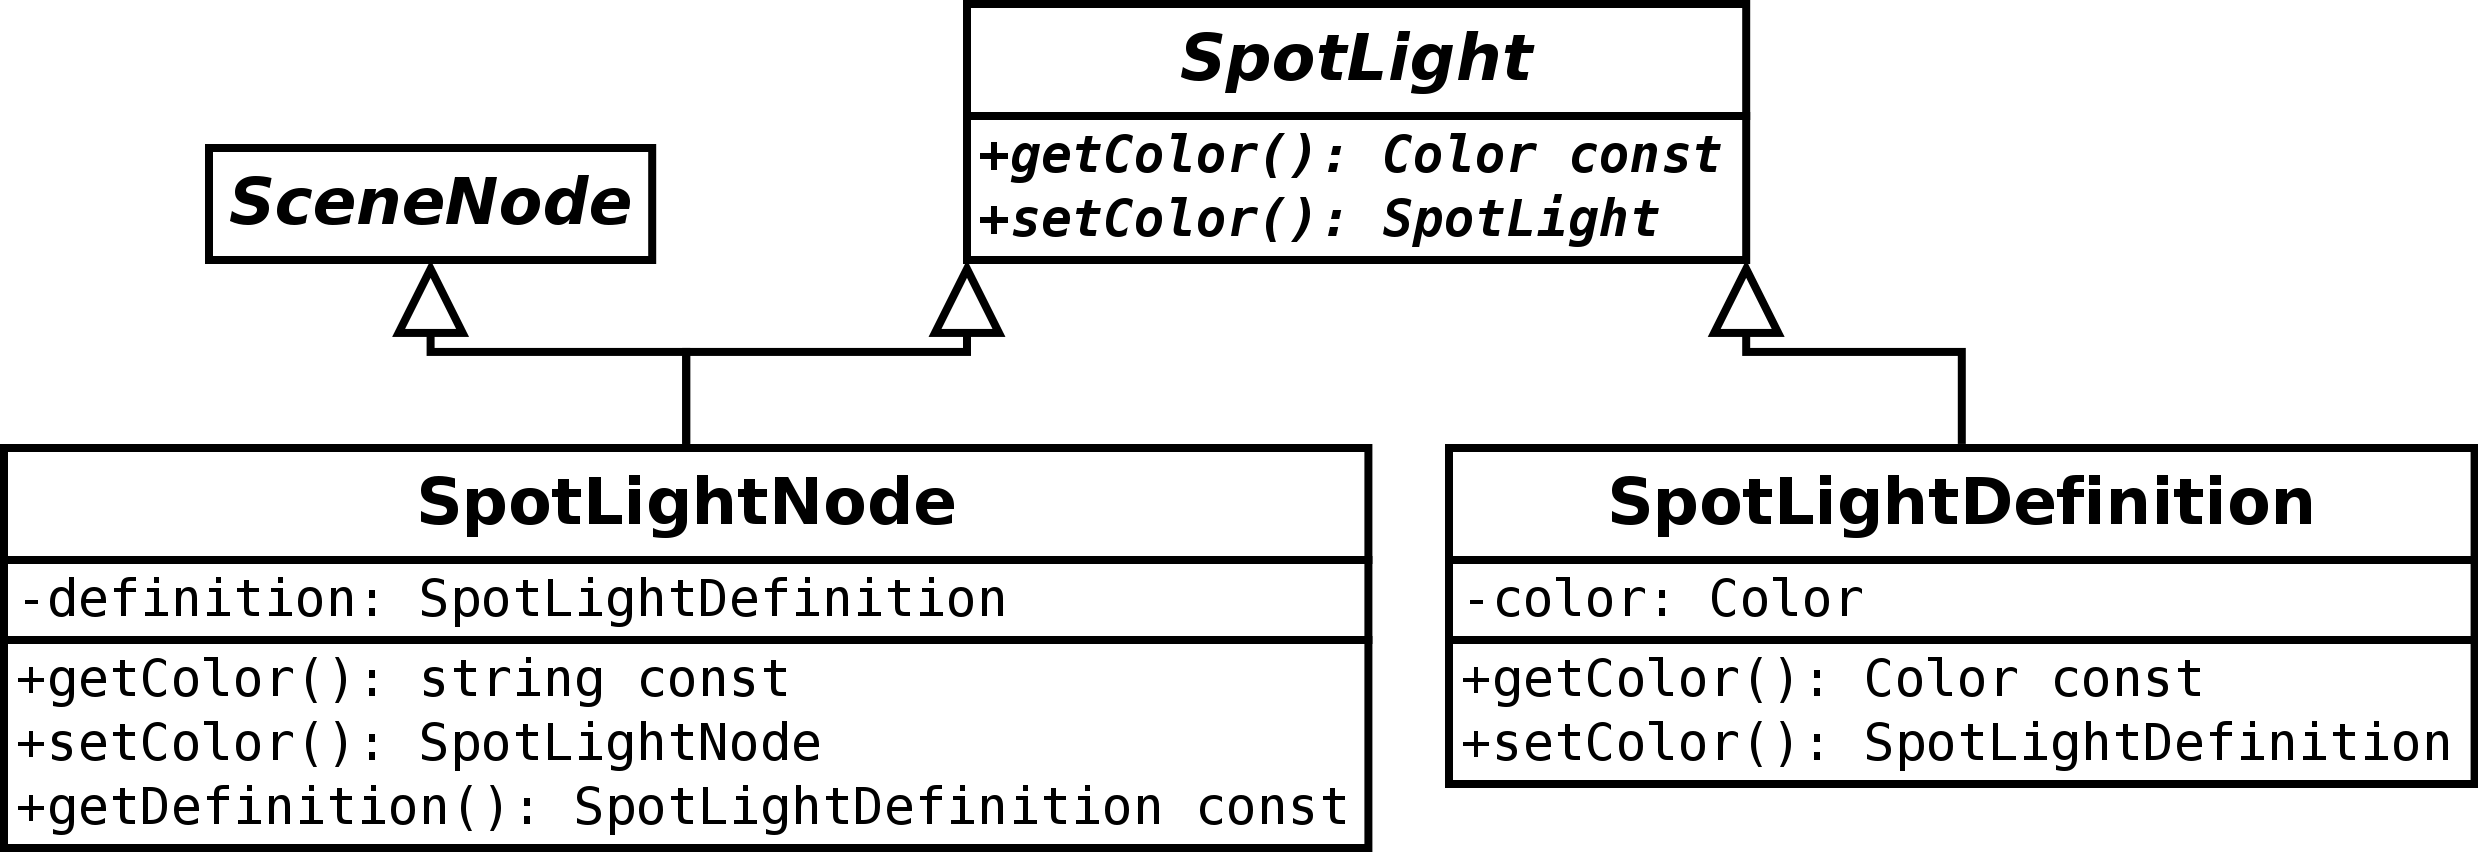
\includegraphics[width=14cm]{images/NodeArchitecture.png}
		\caption{Interdependencies of the three classes required to define and embed a SpotLight into the scene graph.}
		\label{fig:NodeArchitecture}
	\end{figure}

	\begin{smalllist}
		\item The \classname{Definition} defines a re-usable component, such as a single light source in an array of spot lights for the lighting of a theater stage.
		\item The \classname{Node} provides the exact same methods for manipulating the underlying template.
		\item The consequence of this interface is that any operation on the \classname{Node} will alter the appearance of all other nodes in the scene.
	\end{smalllist}

	We can even conceal this distinction between the \classname{Definition} of an object and its integration into the scene via its \classname{Node} class by creating a factory method in the interface. A \classname{SpotLight} is created and embedded in a single step through a call to this factory:

	\begin{code}[2]
		SpotLight* spotLight = SpotLight::create();
	\end{code}

	The \inlinecode{spotLight} created in this example is of type \classname{SpotLightNode} and it contains a pointer to a newly created \classname{SpotLightDefinition}. Creating an array of lights that have the same behavior is accomplished using the factory in \classname{SpotLightNode}:

	% whitespace
	\begin{code}[2]
		std::vector<SpotLight*> lights;
		lights.push_back(SpotLight::create());
		for (int i = 0; i < numLights; i++)
		{
		    lights.push_back(
		        SpotLightNode::create(lights[0]->getDefinition())
		    );
		}
	\end{code}

	With this design, the scene graph has become quite transparent during scene construction:

	\begin{smalllist}
		\item Every created object is immediately attached to the scene graph and
		\item objects can be attached to each other to declare a dependency of their positional properties.
	\end{smalllist}

	There is one scenario left, where attaching objects to each other is not enough to declare a dependency between them. This is the case if the objects involved do not have an intuitive hierarchy between them. In our dinner table example, the association between a fork and a knife is such a case. It is not intuitive to declare either of the objects as the one dictating the position of the other, whereas this approach works in the association between a table and a plate: If we move the table around, we want the plate to keep its position relative to the table, but it is hard to say whether the movement of a fork should affect the knife or vice versa.

	The API so far would require us to create a scene node to provide a common handle for all the cutlery:
	
	\begin{code}[2]
		cutlery = SceneNode::create();
		knife = Model::create("Knife");
		fork = Model::create("Fork");
		knife->attachTo(cutlery);
		fork->attachTo(cutlery);
	\end{code}

	This solution ``leaks'' the existence of a scene graph. This is not a problem per se, but since this is the only scenario in which the scene graph becomes visible in our API, we will try to address this leakage to eliminate yet another new concept in an API providing an introductory portal into an unknown domain.
	
	We will instead use another mental model that is already present in the user interfaces of many applications that need to arrange objects in 2d or 3d space: object groups. This concept is present in many 3d modeling tools\footnote{Some examples of well-established modeling tools are \emph{3d Studio Max}, \emph{Blender} or \emph{Maya}}, as well as in applications for 2d design\footnote{Applications for creating diagrams particularly make use of it, like \emph{dia} or \emph{OmniGraffle}.}.

	An object group has the exact same aim as a node in a scene graph - to introduce a hierarchy into complex object structures. This idea could be implemented in two ways.

	\begin{numlist}
		\item We could either create a \inlinecode{typedef} for the \classname{SceneNode} class, or
		\item declare a sub-class thereof.
	\end{numlist}
	
	We have chosen to create a separate sub-class in order to separate it from the \classname{SceneNode} class. A \inlinecode{typedef} would remove the black-box status of the \classname{SceneNode}. With this last change, the scene graph data structure cannot be found in the API unless one explicitly seeks it out.

